\documentclass[10pt,a4paper,final]{article}
\usepackage[utf8]{inputenc}
\usepackage{tikz}
\usetikzlibrary{quantikz}

\begin{document}

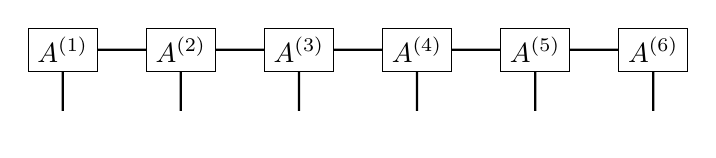
\begin{tikzpicture}[scale=1.5]
\node[draw, shape=rectangle] (A1) at (0,0) {$A^{(1)}$};
\node[draw, shape=rectangle] (A2) at (1,0) {$A^{(2)}$};
\node[draw, shape=rectangle] (A3) at (2,0) {$A^{(3)}$};
\node[draw, shape=rectangle] (A4) at (3,0) {$A^{(4)}$};
\node[draw, shape=rectangle] (A5) at (4,0) {$A^{(5)}$};
\node[draw, shape=rectangle] (A6) at (5,0) {$A^{(6)}$};
\node (B1) at (0,-0.6) {};
\node (B2) at (1,-0.6) {};
\node (B3) at (2,-0.6) {};
\node (B4) at (3,-0.6) {};
\node (B5) at (4,-0.6) {};
\node (B6) at (5,-0.6) {};

\draw [thick] (A1) -- (A2)
(A2) -- (A3)
(A3) -- (A4)
(A4) -- (A5)
(A5) -- (A6)

(A1) -- (B1)
(A2) -- (B2)
(A3) -- (B3)
(A4) -- (B4)
(A5) -- (B5)
(A6) -- (B6);
\end{tikzpicture}

\end{document}